% Options for packages loaded elsewhere
\PassOptionsToPackage{unicode}{hyperref}
\PassOptionsToPackage{hyphens}{url}
\PassOptionsToPackage{dvipsnames,svgnames,x11names}{xcolor}
%
\documentclass[
  11pt,
  letterpaper,
  DIV=11,
  numbers=noendperiod]{scrartcl}

\usepackage{amsmath,amssymb}
\usepackage{lmodern}
\usepackage{iftex}
\ifPDFTeX
  \usepackage[T1]{fontenc}
  \usepackage[utf8]{inputenc}
  \usepackage{textcomp} % provide euro and other symbols
\else % if luatex or xetex
  \usepackage{unicode-math}
  \defaultfontfeatures{Scale=MatchLowercase}
  \defaultfontfeatures[\rmfamily]{Ligatures=TeX,Scale=1}
\fi
% Use upquote if available, for straight quotes in verbatim environments
\IfFileExists{upquote.sty}{\usepackage{upquote}}{}
\IfFileExists{microtype.sty}{% use microtype if available
  \usepackage[]{microtype}
  \UseMicrotypeSet[protrusion]{basicmath} % disable protrusion for tt fonts
}{}
\makeatletter
\@ifundefined{KOMAClassName}{% if non-KOMA class
  \IfFileExists{parskip.sty}{%
    \usepackage{parskip}
  }{% else
    \setlength{\parindent}{0pt}
    \setlength{\parskip}{6pt plus 2pt minus 1pt}}
}{% if KOMA class
  \KOMAoptions{parskip=half}}
\makeatother
\usepackage{xcolor}
\usepackage[margin=2.4cm, footskip=1cm]{geometry}
\setlength{\emergencystretch}{3em} % prevent overfull lines
\setcounter{secnumdepth}{-\maxdimen} % remove section numbering
% Make \paragraph and \subparagraph free-standing
\ifx\paragraph\undefined\else
  \let\oldparagraph\paragraph
  \renewcommand{\paragraph}[1]{\oldparagraph{#1}\mbox{}}
\fi
\ifx\subparagraph\undefined\else
  \let\oldsubparagraph\subparagraph
  \renewcommand{\subparagraph}[1]{\oldsubparagraph{#1}\mbox{}}
\fi

\usepackage{color}
\usepackage{fancyvrb}
\newcommand{\VerbBar}{|}
\newcommand{\VERB}{\Verb[commandchars=\\\{\}]}
\DefineVerbatimEnvironment{Highlighting}{Verbatim}{commandchars=\\\{\}}
% Add ',fontsize=\small' for more characters per line
\usepackage{framed}
\definecolor{shadecolor}{RGB}{241,243,245}
\newenvironment{Shaded}{\begin{snugshade}}{\end{snugshade}}
\newcommand{\AlertTok}[1]{\textcolor[rgb]{0.68,0.00,0.00}{#1}}
\newcommand{\AnnotationTok}[1]{\textcolor[rgb]{0.37,0.37,0.37}{#1}}
\newcommand{\AttributeTok}[1]{\textcolor[rgb]{0.40,0.45,0.13}{#1}}
\newcommand{\BaseNTok}[1]{\textcolor[rgb]{0.68,0.00,0.00}{#1}}
\newcommand{\BuiltInTok}[1]{\textcolor[rgb]{0.00,0.23,0.31}{#1}}
\newcommand{\CharTok}[1]{\textcolor[rgb]{0.13,0.47,0.30}{#1}}
\newcommand{\CommentTok}[1]{\textcolor[rgb]{0.37,0.37,0.37}{#1}}
\newcommand{\CommentVarTok}[1]{\textcolor[rgb]{0.37,0.37,0.37}{\textit{#1}}}
\newcommand{\ConstantTok}[1]{\textcolor[rgb]{0.56,0.35,0.01}{#1}}
\newcommand{\ControlFlowTok}[1]{\textcolor[rgb]{0.00,0.23,0.31}{#1}}
\newcommand{\DataTypeTok}[1]{\textcolor[rgb]{0.68,0.00,0.00}{#1}}
\newcommand{\DecValTok}[1]{\textcolor[rgb]{0.68,0.00,0.00}{#1}}
\newcommand{\DocumentationTok}[1]{\textcolor[rgb]{0.37,0.37,0.37}{\textit{#1}}}
\newcommand{\ErrorTok}[1]{\textcolor[rgb]{0.68,0.00,0.00}{#1}}
\newcommand{\ExtensionTok}[1]{\textcolor[rgb]{0.00,0.23,0.31}{#1}}
\newcommand{\FloatTok}[1]{\textcolor[rgb]{0.68,0.00,0.00}{#1}}
\newcommand{\FunctionTok}[1]{\textcolor[rgb]{0.28,0.35,0.67}{#1}}
\newcommand{\ImportTok}[1]{\textcolor[rgb]{0.00,0.46,0.62}{#1}}
\newcommand{\InformationTok}[1]{\textcolor[rgb]{0.37,0.37,0.37}{#1}}
\newcommand{\KeywordTok}[1]{\textcolor[rgb]{0.00,0.23,0.31}{#1}}
\newcommand{\NormalTok}[1]{\textcolor[rgb]{0.00,0.23,0.31}{#1}}
\newcommand{\OperatorTok}[1]{\textcolor[rgb]{0.37,0.37,0.37}{#1}}
\newcommand{\OtherTok}[1]{\textcolor[rgb]{0.00,0.23,0.31}{#1}}
\newcommand{\PreprocessorTok}[1]{\textcolor[rgb]{0.68,0.00,0.00}{#1}}
\newcommand{\RegionMarkerTok}[1]{\textcolor[rgb]{0.00,0.23,0.31}{#1}}
\newcommand{\SpecialCharTok}[1]{\textcolor[rgb]{0.37,0.37,0.37}{#1}}
\newcommand{\SpecialStringTok}[1]{\textcolor[rgb]{0.13,0.47,0.30}{#1}}
\newcommand{\StringTok}[1]{\textcolor[rgb]{0.13,0.47,0.30}{#1}}
\newcommand{\VariableTok}[1]{\textcolor[rgb]{0.07,0.07,0.07}{#1}}
\newcommand{\VerbatimStringTok}[1]{\textcolor[rgb]{0.13,0.47,0.30}{#1}}
\newcommand{\WarningTok}[1]{\textcolor[rgb]{0.37,0.37,0.37}{\textit{#1}}}

\providecommand{\tightlist}{%
  \setlength{\itemsep}{0pt}\setlength{\parskip}{0pt}}\usepackage{longtable,booktabs,array}
\usepackage{calc} % for calculating minipage widths
% Correct order of tables after \paragraph or \subparagraph
\usepackage{etoolbox}
\makeatletter
\patchcmd\longtable{\par}{\if@noskipsec\mbox{}\fi\par}{}{}
\makeatother
% Allow footnotes in longtable head/foot
\IfFileExists{footnotehyper.sty}{\usepackage{footnotehyper}}{\usepackage{footnote}}
\makesavenoteenv{longtable}
\usepackage{graphicx}
\makeatletter
\def\maxwidth{\ifdim\Gin@nat@width>\linewidth\linewidth\else\Gin@nat@width\fi}
\def\maxheight{\ifdim\Gin@nat@height>\textheight\textheight\else\Gin@nat@height\fi}
\makeatother
% Scale images if necessary, so that they will not overflow the page
% margins by default, and it is still possible to overwrite the defaults
% using explicit options in \includegraphics[width, height, ...]{}
\setkeys{Gin}{width=\maxwidth,height=\maxheight,keepaspectratio}
% Set default figure placement to htbp
\makeatletter
\def\fps@figure{htbp}
\makeatother
\newlength{\cslhangindent}
\setlength{\cslhangindent}{1.5em}
\newlength{\csllabelwidth}
\setlength{\csllabelwidth}{3em}
\newlength{\cslentryspacingunit} % times entry-spacing
\setlength{\cslentryspacingunit}{\parskip}
\newenvironment{CSLReferences}[2] % #1 hanging-ident, #2 entry spacing
 {% don't indent paragraphs
  \setlength{\parindent}{0pt}
  % turn on hanging indent if param 1 is 1
  \ifodd #1
  \let\oldpar\par
  \def\par{\hangindent=\cslhangindent\oldpar}
  \fi
  % set entry spacing
  \setlength{\parskip}{#2\cslentryspacingunit}
 }%
 {}
\usepackage{calc}
\newcommand{\CSLBlock}[1]{#1\hfill\break}
\newcommand{\CSLLeftMargin}[1]{\parbox[t]{\csllabelwidth}{#1}}
\newcommand{\CSLRightInline}[1]{\parbox[t]{\linewidth - \csllabelwidth}{#1}\break}
\newcommand{\CSLIndent}[1]{\hspace{\cslhangindent}#1}

\KOMAoption{captions}{tableheading}
\usepackage{setspace}\onehalfspacing
\setlength{\abovedisplayskip}{4pt}
\setlength{\belowdisplayskip}{4pt}
\setlength{\abovedisplayshortskip}{1pt}
\setlength{\belowdisplayshortskip}{1pt}
\ifdefined\Shaded\renewenvironment{Shaded}{ \small\begin{tcolorbox}[top=2pt, bottom=0pt, borderline west={3pt}{0pt}{shadecolor}, interior hidden, frame hidden, enhanced, boxrule=0pt, sharp corners, breakable]}{\end{tcolorbox}}\fi
\usepackage{pgf}\usepackage{pgfplots}\usepackage{tikz}
\usetikzlibrary{graphs, arrows, automata, shadings}
\setlength{\floatsep}{0pt}
\usepackage{enumitem}\setlist[enumerate]{leftmargin=*}
\usepackage{verbatim}
\makeatletter \patchcmd{\@verbatim}{\verbatim@font}{\singlespacing\small\verbatim@font}{}{}
\makeatletter
\makeatother
\makeatletter
\makeatother
\makeatletter
\@ifpackageloaded{caption}{}{\usepackage{caption}}
\AtBeginDocument{%
\ifdefined\contentsname
  \renewcommand*\contentsname{Table of contents}
\else
  \newcommand\contentsname{Table of contents}
\fi
\ifdefined\listfigurename
  \renewcommand*\listfigurename{List of Figures}
\else
  \newcommand\listfigurename{List of Figures}
\fi
\ifdefined\listtablename
  \renewcommand*\listtablename{List of Tables}
\else
  \newcommand\listtablename{List of Tables}
\fi
\ifdefined\figurename
  \renewcommand*\figurename{Figure}
\else
  \newcommand\figurename{Figure}
\fi
\ifdefined\tablename
  \renewcommand*\tablename{Table}
\else
  \newcommand\tablename{Table}
\fi
}
\@ifpackageloaded{float}{}{\usepackage{float}}
\floatstyle{ruled}
\@ifundefined{c@chapter}{\newfloat{codelisting}{h}{lop}}{\newfloat{codelisting}{h}{lop}[chapter]}
\floatname{codelisting}{Listing}
\newcommand*\listoflistings{\listof{codelisting}{List of Listings}}
\makeatother
\makeatletter
\@ifpackageloaded{caption}{}{\usepackage{caption}}
\@ifpackageloaded{subcaption}{}{\usepackage{subcaption}}
\makeatother
\makeatletter
\@ifpackageloaded{tcolorbox}{}{\usepackage[many]{tcolorbox}}
\makeatother
\makeatletter
\@ifundefined{shadecolor}{\definecolor{shadecolor}{rgb}{.97, .97, .97}}
\makeatother
\makeatletter
\makeatother
\ifLuaTeX
  \usepackage{selnolig}  % disable illegal ligatures
\fi
\IfFileExists{bookmark.sty}{\usepackage{bookmark}}{\usepackage{hyperref}}
\IfFileExists{xurl.sty}{\usepackage{xurl}}{} % add URL line breaks if available
\urlstyle{same} % disable monospaced font for URLs
\hypersetup{
  pdftitle={Progress report},
  pdfauthor={Kevin Chen; Zixuan (Niki) Chen; Lauren Dimaggio; Jingxuan Fan},
  colorlinks=true,
  linkcolor={blue},
  filecolor={Maroon},
  citecolor={Blue},
  urlcolor={Blue},
  pdfcreator={LaTeX via pandoc}}

\title{Progress report}
\author{Kevin Chen \and Zixuan (Niki) Chen \and Lauren
Dimaggio \and Jingxuan Fan}
\date{}

\begin{document}
\maketitle
\ifdefined\Shaded\renewenvironment{Shaded}{\begin{tcolorbox}[interior hidden, frame hidden, breakable, borderline west={3pt}{0pt}{shadecolor}, boxrule=0pt, sharp corners, enhanced]}{\end{tcolorbox}}\fi

All script used to download and clean the data, conduct analyses,
produce output, and prepare documents may be found on our GitHub
repository
\href{https://github.berkeley.edu/kevchen/capstone-epi}{here}. The
repository is organized into five main directories, whose contents
reflect their names:

\begin{itemize}
\tightlist
\item
  \texttt{data} contains raw data as well as cleaned subsets
\item
  \texttt{output} contains descriptive, analytic, and diagnostic results
  as well as intermediate objects produced over the course of work
\item
  \texttt{references} contains scientific/statistical/technical
  literature as well as a BibTeX file enumerating them
\item
  \texttt{reports} contains prepared documents for human consumption and
  the script used to prepare them
\item
  \texttt{script} contains the programming script for all main tasks.
\end{itemize}

The present document describes some of the work done to-date.

\hypertarget{downloading-and-cleaning-data}{%
\section{Downloading and cleaning
data}\label{downloading-and-cleaning-data}}

Data were downloaded directly from the California Health and Human
Services (CalHHS) \href{https://data.chhs.ca.gov}{Open Data Portal}. Two
main datasets were used: (1)
\href{https://data.chhs.ca.gov/dataset/covid-19-time-series-metrics-by-county-and-state}{Statewide
COVID-19 Cases Deaths Tests} and (2)
\href{https://data.chhs.ca.gov/dataset/vaccine-progress-dashboard}{Statewide
COVID-19 Vaccines Administered by County} vaccination counts over time.
Both datasets contain daily time series stratified by county. The script
for downloading the data are saved in file
\texttt{script/download\_data.R} and reproduced below.

\begin{Shaded}
\begin{Highlighting}[]
\CommentTok{\# download\_data.R}
\CommentTok{\# February 9, 2023}
\CommentTok{\# Downloading data from CA Open Data portal}

\FunctionTok{library}\NormalTok{(data.table)}

\CommentTok{\# Case counts}
\NormalTok{cases.url }\OtherTok{\textless{}{-}} \FunctionTok{paste0}\NormalTok{(}
    \StringTok{"https://data.chhs.ca.gov/dataset/"}\NormalTok{,}
    \StringTok{"f333528b{-}4d38{-}4814{-}bebb{-}12db1f10f535/"}\NormalTok{,}
    \StringTok{"resource/"}\NormalTok{,}
    \StringTok{"046cdd2b{-}31e5{-}4d34{-}9ed3{-}b48cdbc4be7a/"}\NormalTok{,}
    \StringTok{"download/covid19cases\_test.csv"}
\NormalTok{)}
\NormalTok{cases.dat }\OtherTok{\textless{}{-}} \FunctionTok{fread}\NormalTok{(cases.url)}
\FunctionTok{write.csv}\NormalTok{(cases.dat, }\StringTok{\textquotesingle{}data/cases.csv\textquotesingle{}}\NormalTok{, }\AttributeTok{row.names =}\NormalTok{ F)}

\CommentTok{\# Vaccination counts}
\NormalTok{vax.url }\OtherTok{\textless{}{-}} \FunctionTok{paste0}\NormalTok{(}
    \StringTok{"https://data.chhs.ca.gov/dataset/"}\NormalTok{,}
    \StringTok{"e283ee5a{-}cf18{-}4f20{-}a92c{-}ee94a2866ccd/"}\NormalTok{,}
    \StringTok{"resource/"}\NormalTok{,}
    \StringTok{"130d7ba2{-}b6eb{-}438d{-}a412{-}741bde207e1c/"}\NormalTok{,}
    \StringTok{"download/covid19vaccinesbycounty.csv"}
\NormalTok{)}
\NormalTok{vax.dat }\OtherTok{\textless{}{-}} \FunctionTok{fread}\NormalTok{(vax.url)}
\FunctionTok{write.csv}\NormalTok{(vax.dat, }\StringTok{\textquotesingle{}data/vax.csv\textquotesingle{}}\NormalTok{, }\AttributeTok{row.names =}\NormalTok{ F)}
\end{Highlighting}
\end{Shaded}

Since the total data are small and clean, minimal processing was
required. We limited the data to days on or after June 15, 2021 to
restrict the analytic problem to the period of time when vaccines were
widely available. The main workhorses for our analysis will be the daily
new case, death, and vaccination counts. While death and vaccination
counts should be accurate (difficult to mis-classify a death and
vaccination requires billing), the case counts may be vulnerable to
changes in reporting and testing. In the next several weeks, we will
explore the use of hospitalization rates, test counts, and test
positivity to construct a more accurate measure of the true case count.

\hypertarget{basic-visualization}{%
\section{Basic visualization}\label{basic-visualization}}

A plot of the daily case counts stratified by county is presented below.
Note that for almost all of the counties that experienced at least
\(10\,000\) cases over the course of available data, there were 4-5
outbreak cycles where the case count underwent exponential growth before
rapidly switching to exponential decay with what appears to be a sudden
change in the velocity. Case count plots for the major counties of
Alameda, San Francisco, Sacramento, Los Angeles, San Diego, and Fresno
are highlighted in their own plot. Despite the differences in the
magnitude of the peaks in the epidemiologic trajectories, the overall
shape of the curves is subjectively similar. The ways in which these
cycles can be represented as parameters of a compartmental model are
discussed below.

\begin{figure}

{\centering \includegraphics{progress_files/figure-pdf/unnamed-chunk-2-1.pdf}

}

\end{figure}

\begin{figure}

{\centering \includegraphics{progress_files/figure-pdf/unnamed-chunk-3-1.pdf}

}

\end{figure}

\hypertarget{basic-epidemiologic-principles-and-compartmental-modeling.}{%
\section{Basic epidemiologic principles and compartmental
modeling.}\label{basic-epidemiologic-principles-and-compartmental-modeling.}}

The study of disease distributions and infectious disease transmission
have long be central to public health research and practice. Before the
wide acceptance of germ theory, early epidemiologists such as John Snow
identified causes of health and disease by analyzing binary contrasts in
exposure status without a clear model of the biological manifestation of
those exposures (Vinten-Johansen et al. 2003). By the 1910s, physicians
and researchers became comfortable with the notion of the \emph{natural
history of disease} ie the progression of a disease process in an
individual over time. The most basic conceptualization of the natural
history of an infectious disease is an individual's progression from
susceptibility to infected and finally, recovery. This model forms the
basis for one of the simplest of compartmental models used for modeling
disease trajectory in a population: the \(SIR\) model (Harko, Lobo, and
Mak 2014). The flow of individuals through the states in a closed
population is modeled as systems of ordinary differential equations:
\[\left\{
\begin{aligned}
\frac{d}{dt} S & = - \frac{\beta}{N} I S \\
\frac{d}{dt} I & = \frac{\beta}{N} I S  -  \gamma I \\
\frac{d}{dt} R & = \gamma I
\end{aligned}
\right.\]

This approach gives rise to parameters that are convenient for both
estimation and interpretation. The transmission parameter \(\beta\) and
the force of infection \(\gamma\) represent rates of change of the \(S\)
and \(I\) states respectively. The transmission parameter and the force
of infection are related through a constant \(R_0\) such that
\(\beta = R_0 \times \gamma\) where \(R_0\) may be interpreted as the
average number of new cases (infections) that arise from contact with a
case. This parameter is known as the basic reproduction number.

\begin{figure}[H]
\caption{$SIR$ model.}
\begin{center}
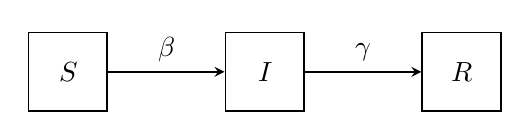
\begin{tikzpicture}[>= stealth, shorten >= 0pt,
                    auto, node distance=2.5cm, semithick]
\tikzstyle{every state}=[shape=rectangle, draw=black, 
                    semithick, inner sep=1pt, minimum size=1cm]
  \node[state] (S) {$S$};
  \node[state] (I) [right of=S] {$I$};
  \node[state] (R)   [right of=I] {$R$};
  \path[->]    (S) edge node {$\beta$} (I);
  \path[->]    (I) edge node {$\gamma$} (R);
\end{tikzpicture}
\end{center}
\end{figure}

\hypertarget{solutions-at-analyst-defined-parameter-values}{%
\section{Solutions at analyst-defined parameter
values}\label{solutions-at-analyst-defined-parameter-values}}

Well known extensions of the \(SIR\) model include \(SIRS\), \(SEIR\)
and \(SEIRS\) (Vynnycky and White 2010, 16). One extension presented by
Rella et al. (2021) included five additional compartments to account for
vaccination, transmission of a vaccine-resistant strain, and death.
Under that compartmental model, emergence of a vaccine-resistant strain
was governed by a rate parameter \(p\), which served as a rate parameter
for the instantaneous emergence of a vaccine-resistant strain among
those infected with a wild type (non-resistant) strain. Note that
setting \(p = 0\) results in a four compartment \(SIRD\) model with an
additional compartment \(V\) for vaccination. Below, we present the
ordinary differential equations for the model presented by Rella et al.
(2021), but further extended to allow for flow from the vaccinated
compartment back into the susceptible compartment with rate \(\omega\).
Note that here, we take \(\beta \times N\) to be the transmission
parameter.

\[\left\{
\begin{aligned}
\frac{d}{dt}  S 
        & = \mu R + \omega V - \theta S - \beta (I_{wt} + I_r + I_{r}^V)  S \\
\frac{d}{dt}  I_{wt} 
        & = - (\gamma + \delta)  I_{wt} + \beta  S  (I_{wt}) \\
\frac{d}{dt}  I_r
        & = - (\gamma + \delta)  I_r  + \beta  S  (I_r + I_r^V) \\
\frac{d}{dt}  I_r^V
        & = - (\gamma + \delta)  I_r^V + \beta  V  (I_r + I_r^V) \\
\frac{d}{dt}  R
        & = - \mu  R - \theta  R + \gamma  (I_{wt} + I_r) \\
\frac{d}{dt}  R^V
        & = - \mu  R^V + \theta  R + \gamma  I_r^V \\ 
\frac{d}{dt}  D
        & = \delta  (I_{wt} + I_r + I_r^V) \\
\frac{d}{dt}  V
    & = \mu  R^V + \theta  S - \beta  V + (I_r + I_r^V) - \omega V
\end{aligned}
\right.\]

\begin{figure}[h]
\caption{Compartmental model of Rella et alia (2021), extended to allow vaccinated individuals to return to being susceptible.}
\begin{center}
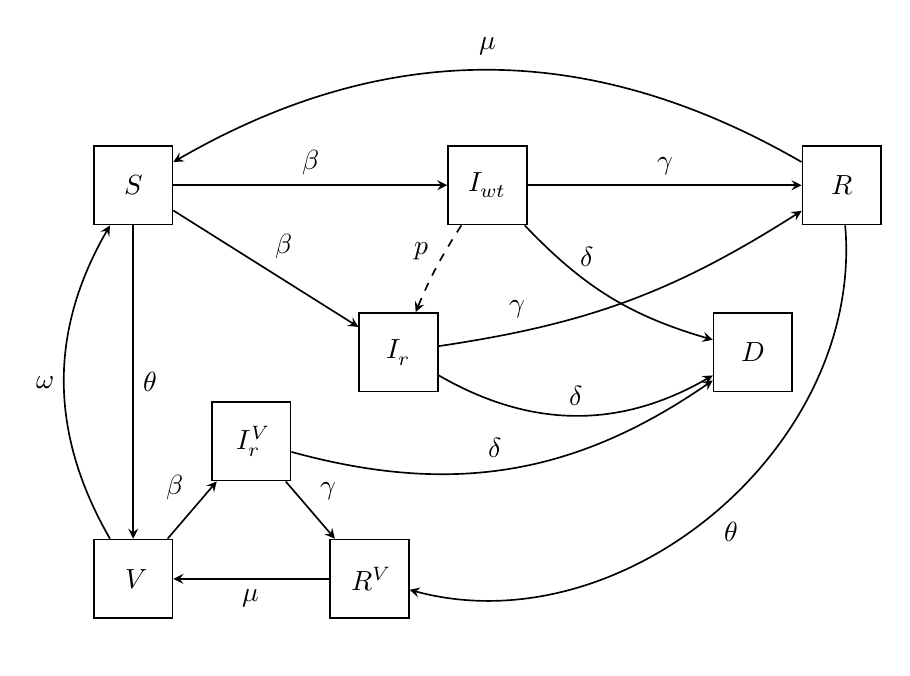
\begin{tikzpicture}[>= stealth, shorten >= 0pt,
                    auto, node distance=4.5cm, semithick]
\tikzstyle{every state}=[shape=rectangle, draw=black, 
                    semithick, inner sep=1pt, minimum size=1cm]
  \node[state] (S) {$S$};
  \node[state] (Iwt) [right of=S] {$I_{wt}$};
  \node[state] (R)   [right of=Iwt] {$R$};
  \node[state] (Ir)  [below right of=S, node distance=3cm, xshift=1.25cm] {$I_r$};
  \node[state] (D)   [right of=Ir] {$D$};
  \node[state] (V)   [below of=S, node distance=5cm] {$V$};
  \node[state] (IrV) [above right of=V, node distance=2.12cm, yshift=0.25cm] {$I_r^V$};
  \node[state] (RV)  [right of=V, node distance=3cm] {$R^V$};
  \path[->]    (S)   edge node {$\beta$} (Iwt);
  \path[->]    (S)   edge node {$\theta$} (V);
  \path[->]    (Iwt) edge node {$\gamma$} (R);
  \path[->]    (R)   edge [bend right=30] node [yshift=0.55cm] {$\mu$} (S);
  \path[->]    (Iwt) edge [bend right=15] node [yshift=0.25cm,xshift=-0.5cm] {$\delta$} (D);
  \path[->]    (R)   edge [bend left=55] node {$\theta$} (RV);
  \path[->]    (RV)  edge node {$\mu$} (V);
  \path[->]    (V)   edge node {$\beta$} (IrV);
  \path[->]    (IrV) edge node {$\gamma$} (RV);
  \path[->]    (IrV) edge [bend right=25] node {$\delta$} (D);
  \path[->]    (S)   edge node {$\beta$} (Ir);
  \path[->]    (Ir)  edge [bend right=12] node [yshift=-0.35cm, xshift=-1.2cm] {$\gamma$} (R);
  \path[->]    (Ir)  edge [bend right=30] node {$\delta$} (D);
  \path[->]    (Iwt) edge [style=dashed, bend right=5] node [yshift=0.45cm, xshift=-0.4cm] {$p$} (Ir);
  \path[->]    (V) edge [bend left=30] node {$\omega$} (S);
\end{tikzpicture}
\end{center}
\end{figure}

The waves in the disease trajectory over time may be captured by a
time-varying reproduction number. Rella et al. (2021) defined two basic
reproduction numbers, one for exponential growth and one for exponential
decay. They theorized that the disease trajectory would begin with a
period of exponential growth until the prevalence of disease reaches
\(F_h\), when the basic reproduction number would switch to one below 1.
This period of exponential decay would resume until the prevalence is at
the low threshold \(F_l\). This conceptualization of the relationship
between the transmission parameter and time makes sense because the
outbreak cycles do not appear to have smooth second derivatives.
Differences in heights of the outbreak cycles may be explained by
different thresholds \(F_h\) and \(F_l\) over different time periods.

\hypertarget{solutions-at-analyst-defined-parameter-values-1}{%
\section{Solutions at analyst-defined parameter
values}\label{solutions-at-analyst-defined-parameter-values-1}}

We encoded the ordinary differential equations described in the previous
section in the file \texttt{script/01-compartments.R} (and below). In
addition to the differential equations wrapped in the function
\texttt{compartmetal\_model()}, we also have helper function
\texttt{get\_beta()}, for computing the time-varying value of the
transmission parameter based on the prevalence of disease (sum of the
\(I\) compartments). The value of the transmission parameter is
necessary for predicting new cases on each day:
\[\text{new cases} = \beta \big(
S (I_{wt} + I_r + I_r^V) + V (I_r + I_r^V)
\big)\] For San Francisco (\(N = 815\,201\)), we can plot the solution
of the model above given plausible (but arbitrarily specified) parameter
values.

\begin{longtable}[]{@{}
  >{\raggedright\arraybackslash}p{(\columnwidth - 4\tabcolsep) * \real{0.1625}}
  >{\raggedright\arraybackslash}p{(\columnwidth - 4\tabcolsep) * \real{0.2750}}
  >{\raggedright\arraybackslash}p{(\columnwidth - 4\tabcolsep) * \real{0.5625}}@{}}
\toprule()
\begin{minipage}[b]{\linewidth}\raggedright
Parameter
\end{minipage} & \begin{minipage}[b]{\linewidth}\raggedright
Value
\end{minipage} & \begin{minipage}[b]{\linewidth}\raggedright
Interpretation
\end{minipage} \\
\midrule()
\endhead
\(\theta\) & 250.6335 & Vaccination rate (vaccines per day) \\
\(\delta\) & 7.3 \(\times\) 10,000 & Death rate (deaths per day) \\
\({R_0}_h\) & 2.2 & Basic reproduction number during growth \\
\({R_0}_l\) & 0.65 & Basic reproduction number during decay \\
\(\gamma\) & 1 / 14 & Inverse disease duration (days) \\
\(\mu\) & 1 / (30 \(\times\) 12) & Inverse duration of natural
immunity \\
\(\omega\) & 1 / (30 \(\times\) 12) & Inverse duration of vaccine
protection \\
\(p_{h,1}\) & 1 / 350 & Maximum prevalence before preventive measures in
first wave \\
\(p_{h,2}\) & 1 / 63 & Maximum prevalence in second wave \\
\(p_{h,3}\) & 1 / 165 & Maximum prevalence in third wave \\
\(p_{h,4}\) & 1 / 325 & Maximum prevalence in fourth wave \\
\(p_{l,1}\) & 1 / (350 \(\times\) 15) & Allowable prevalence before
before loosening measures (1st) \\
\(p_{l,2}\) & 1 / (63 \(\times\) 15) & Allowable prevalence (2nd) \\
\(p_{l,3}\) & 1 / (165 \(\times\) 2.5) & Allowable prevalence (3rd) \\
\(p_{l,4}\) & 1 / (325 \(\times\) 17) & Allowable prevalence (4th) \\
\bottomrule()
\end{longtable}

The script for plotting a deterministic solution with these parameters
can be found in \texttt{script/eyeball-fit.R} (and below). Such a plot
is presented below with the salmon-colored line representing the
predicted incidence and the points reprenting the observed new case
count.

\begin{verbatim}
-- Attaching packages --------------------------------------- tidyverse 1.3.2 --
v tibble  3.1.8     v dplyr   1.1.0
v tidyr   1.3.0     v stringr 1.5.0
v readr   2.1.3     v forcats 0.5.2
v purrr   1.0.1     
-- Conflicts ------------------------------------------ tidyverse_conflicts() --
x dplyr::between()   masks data.table::between()
x dplyr::filter()    masks stats::filter()
x dplyr::first()     masks data.table::first()
x dplyr::lag()       masks stats::lag()
x dplyr::last()      masks data.table::last()
x purrr::transpose() masks data.table::transpose()
\end{verbatim}

\begin{figure}

{\centering \includegraphics{progress_files/figure-pdf/unnamed-chunk-4-1.pdf}

}

\end{figure}

\begin{Shaded}
\begin{Highlighting}[]
\CommentTok{\# state\_model.R}
\CommentTok{\# February 9, 2023}
\CommentTok{\# Simple ODE implementation}

\FunctionTok{library}\NormalTok{(tidyverse)}
\FunctionTok{library}\NormalTok{(data.table)}
\FunctionTok{library}\NormalTok{(deSolve)}

\CommentTok{\# \textasciitilde{}\textasciitilde{}\textasciitilde{}\textasciitilde{}\textasciitilde{}\textasciitilde{}\textasciitilde{}\textasciitilde{}\textasciitilde{}\textasciitilde{}\textasciitilde{}\textasciitilde{}\textasciitilde{}\textasciitilde{}\textasciitilde{}\textasciitilde{}\textasciitilde{}\textasciitilde{}\textasciitilde{}\textasciitilde{}\textasciitilde{}\textasciitilde{}\textasciitilde{}\textasciitilde{}\textasciitilde{}\textasciitilde{}\textasciitilde{}\textasciitilde{}\textasciitilde{}\textasciitilde{}\textasciitilde{}\textasciitilde{}\textasciitilde{}\textasciitilde{}\textasciitilde{}\textasciitilde{}\textasciitilde{}\textasciitilde{}\textasciitilde{}\textasciitilde{}\textasciitilde{}\textasciitilde{}\textasciitilde{}\textasciitilde{}\textasciitilde{}\textasciitilde{}\textasciitilde{}\textasciitilde{}\textasciitilde{}\textasciitilde{}\textasciitilde{}\textasciitilde{}\textasciitilde{}\textasciitilde{}\textasciitilde{}\textasciitilde{}\textasciitilde{}\textasciitilde{}\textasciitilde{}\textasciitilde{}\textasciitilde{}\textasciitilde{}\textasciitilde{}\textasciitilde{}\textasciitilde{}\textasciitilde{}\textasciitilde{}\textasciitilde{}\textasciitilde{}\textasciitilde{}\textasciitilde{}\textasciitilde{}\textasciitilde{}\textasciitilde{}\textasciitilde{}\textasciitilde{}\textasciitilde{}\textasciitilde{}}
\CommentTok{\# Derivatives function for closed compartmental model:}
\CommentTok{\# \textasciitilde{}\textasciitilde{}\textasciitilde{}\textasciitilde{}\textasciitilde{}\textasciitilde{}\textasciitilde{}\textasciitilde{}\textasciitilde{}\textasciitilde{}\textasciitilde{}\textasciitilde{}\textasciitilde{}\textasciitilde{}\textasciitilde{}\textasciitilde{}\textasciitilde{}\textasciitilde{}\textasciitilde{}\textasciitilde{}\textasciitilde{}\textasciitilde{}\textasciitilde{}\textasciitilde{}\textasciitilde{}\textasciitilde{}\textasciitilde{}\textasciitilde{}\textasciitilde{}\textasciitilde{}\textasciitilde{}\textasciitilde{}\textasciitilde{}\textasciitilde{}\textasciitilde{}\textasciitilde{}\textasciitilde{}\textasciitilde{}\textasciitilde{}\textasciitilde{}\textasciitilde{}\textasciitilde{}\textasciitilde{}\textasciitilde{}\textasciitilde{}\textasciitilde{}\textasciitilde{}\textasciitilde{}\textasciitilde{}\textasciitilde{}\textasciitilde{}\textasciitilde{}\textasciitilde{}\textasciitilde{}\textasciitilde{}\textasciitilde{}\textasciitilde{}\textasciitilde{}\textasciitilde{}\textasciitilde{}\textasciitilde{}\textasciitilde{}\textasciitilde{}\textasciitilde{}\textasciitilde{}\textasciitilde{}\textasciitilde{}\textasciitilde{}\textasciitilde{}\textasciitilde{}\textasciitilde{}\textasciitilde{}\textasciitilde{}\textasciitilde{}\textasciitilde{}\textasciitilde{}\textasciitilde{}\textasciitilde{}}
\NormalTok{compartmental\_model }\OtherTok{\textless{}{-}} \ControlFlowTok{function}\NormalTok{(time, }\AttributeTok{state =}\NormalTok{ initial\_state, parameters) \{}
    \CommentTok{\# Parameters:}
\NormalTok{    F\_h     }\OtherTok{\textless{}{-}}\NormalTok{ parameters[}\StringTok{\textquotesingle{}F\_h\textquotesingle{}}\NormalTok{]}
\NormalTok{    gamma   }\OtherTok{\textless{}{-}} \DecValTok{1} \SpecialCharTok{/}\NormalTok{ parameters[}\StringTok{"disease\_duration"}\NormalTok{]}
\NormalTok{    delta   }\OtherTok{\textless{}{-}}\NormalTok{ parameters[}\StringTok{"death\_rate"}\NormalTok{]}
\NormalTok{    theta0  }\OtherTok{\textless{}{-}}\NormalTok{ parameters[}\StringTok{"vaccination\_rate"}\NormalTok{]}
\NormalTok{    w       }\OtherTok{\textless{}{-}} \DecValTok{1} \SpecialCharTok{/}\NormalTok{ parameters[}\StringTok{"immune\_period"}\NormalTok{]}
\NormalTok{    mu      }\OtherTok{\textless{}{-}} \DecValTok{1} \SpecialCharTok{/}\NormalTok{ parameters[}\StringTok{"recovery\_period"}\NormalTok{]}
\NormalTok{    p       }\OtherTok{\textless{}{-}} \DecValTok{0}
\NormalTok{    R0\_high }\OtherTok{\textless{}{-}}\NormalTok{ parameters[}\StringTok{"R0\_high"}\NormalTok{]}
\NormalTok{    R0\_low  }\OtherTok{\textless{}{-}}\NormalTok{ parameters[}\StringTok{"R0\_low"}\NormalTok{]}
\NormalTok{    tighten\_factor1   }\OtherTok{\textless{}{-}}\NormalTok{ parameters[}\StringTok{"tighten\_factor1"}\NormalTok{]}
\NormalTok{    tighten\_factor2   }\OtherTok{\textless{}{-}}\NormalTok{ parameters[}\StringTok{"tighten\_factor2"}\NormalTok{]}
\NormalTok{    tighten\_factor3   }\OtherTok{\textless{}{-}}\NormalTok{ parameters[}\StringTok{"tighten\_factor3"}\NormalTok{]}
\NormalTok{    tighten\_factor4   }\OtherTok{\textless{}{-}}\NormalTok{ parameters[}\StringTok{"tighten\_factor4"}\NormalTok{]}
\NormalTok{    loosen\_factor1   }\OtherTok{\textless{}{-}}\NormalTok{ parameters[}\StringTok{"loosen\_factor1"}\NormalTok{]}
\NormalTok{    loosen\_factor2   }\OtherTok{\textless{}{-}}\NormalTok{ parameters[}\StringTok{"loosen\_factor2"}\NormalTok{]}
\NormalTok{    loosen\_factor3   }\OtherTok{\textless{}{-}}\NormalTok{ parameters[}\StringTok{"loosen\_factor3"}\NormalTok{]}
\NormalTok{    loosen\_factor4   }\OtherTok{\textless{}{-}}\NormalTok{ parameters[}\StringTok{"loosen\_factor4"}\NormalTok{]}
    \CommentTok{\# as.integer(as.Date(\textquotesingle{}2021{-}11{-}21\textquotesingle{}) {-} as.Date(\textquotesingle{}2021{-}06{-}14\textquotesingle{}))}
\NormalTok{    holiday\_date     }\OtherTok{\textless{}{-}}\NormalTok{ parameters[}\StringTok{"holiday\_date"}\NormalTok{]}
    \CommentTok{\# as.integer(as.Date(\textquotesingle{}2022{-}04{-}15\textquotesingle{}) {-} as.Date(\textquotesingle{}2021{-}06{-}14\textquotesingle{}))}
\NormalTok{    reopening\_date   }\OtherTok{\textless{}{-}}\NormalTok{ parameters[}\StringTok{"reopening\_date"}\NormalTok{]}
    \CommentTok{\# as.integer(as.Date(\textquotesingle{}2022{-}07{-}04\textquotesingle{}) {-} as.Date(\textquotesingle{}2021{-}06{-}14\textquotesingle{}))}
\NormalTok{    summer\_date      }\OtherTok{\textless{}{-}}\NormalTok{ parameters[}\StringTok{"summer\_date"}\NormalTok{]}
\NormalTok{    emergence\_date      }\OtherTok{\textless{}{-}}\NormalTok{ parameters[}\StringTok{"emergence\_date"}\NormalTok{]}
\NormalTok{    h       }\OtherTok{\textless{}{-}}\NormalTok{ parameters[}\StringTok{"p\_non\_vax"}\NormalTok{]}
\NormalTok{    k       }\OtherTok{\textless{}{-}}\NormalTok{ parameters[}\StringTok{"saturation"}\NormalTok{]}
\NormalTok{    dt      }\OtherTok{\textless{}{-}}\NormalTok{ parameters[}\StringTok{"dt"}\NormalTok{]}
\NormalTok{    R0     }\OtherTok{\textless{}{-}} \FunctionTok{get}\NormalTok{(}\StringTok{\textquotesingle{}R0\textquotesingle{}}\NormalTok{, }\AttributeTok{envir =}\NormalTok{ .GlobalEnv)}
    \CommentTok{\# States:}
\NormalTok{    S    }\OtherTok{\textless{}{-}}\NormalTok{ state[}\StringTok{"S"}\NormalTok{]}
\NormalTok{    I\_wt }\OtherTok{\textless{}{-}}\NormalTok{ state[}\StringTok{"I\_wt"}\NormalTok{]}
\NormalTok{    I\_r  }\OtherTok{\textless{}{-}}\NormalTok{ state[}\StringTok{\textquotesingle{}I\_r\textquotesingle{}}\NormalTok{]}
\NormalTok{    I\_rV }\OtherTok{\textless{}{-}}\NormalTok{ state[}\StringTok{"I\_rV"}\NormalTok{]}
\NormalTok{    R    }\OtherTok{\textless{}{-}}\NormalTok{ state[}\StringTok{"R"}\NormalTok{]}
\NormalTok{    RV   }\OtherTok{\textless{}{-}}\NormalTok{ state[}\StringTok{"RV"}\NormalTok{]}
\NormalTok{    D    }\OtherTok{\textless{}{-}}\NormalTok{ state[}\StringTok{"D"}\NormalTok{]}
\NormalTok{    V    }\OtherTok{\textless{}{-}}\NormalTok{ state[}\StringTok{"V"}\NormalTok{]}
\NormalTok{    N }\OtherTok{\textless{}{-}}\NormalTok{  S }\SpecialCharTok{+}\NormalTok{ I\_wt }\SpecialCharTok{+}\NormalTok{ I\_r }\SpecialCharTok{+}\NormalTok{ I\_rV }\SpecialCharTok{+}\NormalTok{ R }\SpecialCharTok{+}\NormalTok{ RV }\SpecialCharTok{+}\NormalTok{ D }\SpecialCharTok{+}\NormalTok{ V}
    \CommentTok{\# Time{-}varying parameters}
    \DocumentationTok{\#\# Vaccination rate}
\NormalTok{    theta }\OtherTok{\textless{}{-}}\NormalTok{ (}\DecValTok{1} \SpecialCharTok{{-}}\NormalTok{ h }\SpecialCharTok{/}\NormalTok{ (S }\SpecialCharTok{+}\NormalTok{ R }\SpecialCharTok{+}\NormalTok{ I\_wt }\SpecialCharTok{+}\NormalTok{ I\_r)) }\SpecialCharTok{*}\NormalTok{ theta0 }\SpecialCharTok{/}\NormalTok{ (S }\SpecialCharTok{+}\NormalTok{ R }\SpecialCharTok{+}\NormalTok{ k)}
    \DocumentationTok{\#\# Time{-}varying force of  infection}
    \ControlFlowTok{if}\NormalTok{ (time }\SpecialCharTok{\textgreater{}} \DecValTok{0}\NormalTok{)   \{F\_h }\OtherTok{\textless{}{-}}\NormalTok{ N }\SpecialCharTok{/}\NormalTok{ tighten\_factor1; loosen\_factor }\OtherTok{\textless{}{-}}\NormalTok{ loosen\_factor1\}}
    \ControlFlowTok{if}\NormalTok{ (time }\SpecialCharTok{\textgreater{}=}\NormalTok{ holiday\_date) \{}
\NormalTok{        F\_h }\OtherTok{\textless{}{-}}\NormalTok{ N }\SpecialCharTok{/}\NormalTok{ tighten\_factor2; loosen\_factor }\OtherTok{\textless{}{-}}\NormalTok{ loosen\_factor2\}}
    \ControlFlowTok{if}\NormalTok{ (time }\SpecialCharTok{\textgreater{}=}\NormalTok{ reopening\_date) \{}
\NormalTok{        F\_h }\OtherTok{\textless{}{-}}\NormalTok{ N }\SpecialCharTok{/}\NormalTok{ tighten\_factor3; loosen\_factor }\OtherTok{\textless{}{-}}\NormalTok{ loosen\_factor3\}}
    \ControlFlowTok{if}\NormalTok{ (time }\SpecialCharTok{\textgreater{}=}\NormalTok{ summer\_date) \{}
\NormalTok{        F\_h }\OtherTok{\textless{}{-}}\NormalTok{ N }\SpecialCharTok{/}\NormalTok{ tighten\_factor4; loosen\_factor }\OtherTok{\textless{}{-}}\NormalTok{ loosen\_factor4\}}
    \ControlFlowTok{if}\NormalTok{ ((I\_wt }\SpecialCharTok{+}\NormalTok{ I\_r }\SpecialCharTok{+}\NormalTok{ I\_rV) }\SpecialCharTok{\textgreater{}}\NormalTok{ F\_h }\SpecialCharTok{\&}\NormalTok{ R0 }\SpecialCharTok{\textgreater{}}\NormalTok{ R0\_low)                   \{R0 }\OtherTok{\textless{}\textless{}{-}}\NormalTok{ R0\_low\}}
    \ControlFlowTok{if}\NormalTok{ ((I\_wt }\SpecialCharTok{+}\NormalTok{ I\_r }\SpecialCharTok{+}\NormalTok{ I\_rV) }\SpecialCharTok{\textless{}}\NormalTok{ (F\_h }\SpecialCharTok{/}\NormalTok{ loosen\_factor) }\SpecialCharTok{\&}\NormalTok{ R0 }\SpecialCharTok{\textless{}}\NormalTok{ R0\_high)  \{R0 }\OtherTok{\textless{}\textless{}{-}}\NormalTok{ R0\_high\}}
\NormalTok{    beta  }\OtherTok{\textless{}{-}} \FunctionTok{get}\NormalTok{(}\StringTok{\textquotesingle{}R0\textquotesingle{}}\NormalTok{, }\AttributeTok{envir =}\NormalTok{ .GlobalEnv) }\SpecialCharTok{*}\NormalTok{ gamma }\SpecialCharTok{/}\NormalTok{ N}
    \CommentTok{\# Resistant strain?}
    \ControlFlowTok{if}\NormalTok{ ((I\_r }\SpecialCharTok{+}\NormalTok{ I\_rV) }\SpecialCharTok{\textless{}=} \DecValTok{1000} \SpecialCharTok{*}\NormalTok{ N }\SpecialCharTok{\&}\NormalTok{ time }\SpecialCharTok{\textgreater{}=}\NormalTok{ emergence\_date) \{}
\NormalTok{        p }\OtherTok{\textless{}{-}}\NormalTok{ parameters[}\StringTok{\textquotesingle{}emergence\_rate\textquotesingle{}}\NormalTok{]}
            \ControlFlowTok{if}\NormalTok{ (parameters[}\StringTok{\textquotesingle{}stochastic\textquotesingle{}}\NormalTok{]) \{}
\NormalTok{            n\_to\_r  }\OtherTok{\textless{}\textless{}{-}} \FunctionTok{rpois}\NormalTok{(}\DecValTok{1}\NormalTok{, dt }\SpecialCharTok{*}\NormalTok{ p }\SpecialCharTok{*} \FunctionTok{max}\NormalTok{(}\DecValTok{0}\NormalTok{, I\_wt))}
\NormalTok{            n\_to\_wt }\OtherTok{\textless{}\textless{}{-}} \FunctionTok{rpois}\NormalTok{(}\DecValTok{1}\NormalTok{, dt }\SpecialCharTok{*}\NormalTok{ p }\SpecialCharTok{*} \FunctionTok{max}\NormalTok{(}\DecValTok{0}\NormalTok{, I\_r))}
\NormalTok{            \} }\ControlFlowTok{else}\NormalTok{ \{}
\NormalTok{                n\_to\_r  }\OtherTok{\textless{}\textless{}{-}}\NormalTok{ dt }\SpecialCharTok{*}\NormalTok{ p }\SpecialCharTok{*} \FunctionTok{max}\NormalTok{(}\DecValTok{0}\NormalTok{, I\_wt)}
\NormalTok{                n\_to\_wt }\OtherTok{\textless{}\textless{}{-}}\NormalTok{ dt }\SpecialCharTok{*}\NormalTok{ p }\SpecialCharTok{*} \FunctionTok{max}\NormalTok{(}\DecValTok{0}\NormalTok{, I\_r)}
\NormalTok{            \}}
\NormalTok{        I\_r  }\OtherTok{\textless{}{-}}\NormalTok{ I\_r  }\SpecialCharTok{{-}}\NormalTok{ n\_to\_wt }\SpecialCharTok{+}\NormalTok{ n\_to\_r}
\NormalTok{        I\_wt }\OtherTok{\textless{}{-}}\NormalTok{ I\_wt }\SpecialCharTok{+}\NormalTok{ n\_to\_wt }\SpecialCharTok{{-}}\NormalTok{ n\_to\_r}
\NormalTok{    \}}
    \CommentTok{\# Derivatives:}
\NormalTok{    dS    }\OtherTok{\textless{}{-}}\NormalTok{ mu }\SpecialCharTok{*}\NormalTok{ R }\SpecialCharTok{+}\NormalTok{ w }\SpecialCharTok{*}\NormalTok{ V }\SpecialCharTok{{-}}\NormalTok{ theta }\SpecialCharTok{*}\NormalTok{ S }\SpecialCharTok{{-}}\NormalTok{ beta }\SpecialCharTok{*}\NormalTok{ (I\_wt }\SpecialCharTok{+}\NormalTok{ I\_r }\SpecialCharTok{+}\NormalTok{ I\_rV) }\SpecialCharTok{*}\NormalTok{ S}
\NormalTok{    dI\_wt }\OtherTok{\textless{}{-}} \SpecialCharTok{{-}}\NormalTok{ (gamma }\SpecialCharTok{+}\NormalTok{ delta) }\SpecialCharTok{*}\NormalTok{ I\_wt }\SpecialCharTok{+}\NormalTok{ beta }\SpecialCharTok{*}\NormalTok{ S }\SpecialCharTok{*}\NormalTok{ (I\_wt)}
\NormalTok{    dI\_r  }\OtherTok{\textless{}{-}}\NormalTok{ (}\SpecialCharTok{{-}}\NormalTok{ (gamma }\SpecialCharTok{+}\NormalTok{ delta) }\SpecialCharTok{*}\NormalTok{ I\_r  }\SpecialCharTok{+}\NormalTok{ beta }\SpecialCharTok{*}\NormalTok{ S }\SpecialCharTok{*}\NormalTok{ (I\_r }\SpecialCharTok{+}\NormalTok{ I\_rV))}
\NormalTok{    dI\_rV }\OtherTok{\textless{}{-}} \SpecialCharTok{{-}}\NormalTok{ (gamma }\SpecialCharTok{+}\NormalTok{ delta) }\SpecialCharTok{*}\NormalTok{ I\_rV }\SpecialCharTok{+}\NormalTok{ beta }\SpecialCharTok{*}\NormalTok{ V }\SpecialCharTok{*}\NormalTok{ (I\_r }\SpecialCharTok{+}\NormalTok{ I\_rV)}
\NormalTok{    dR    }\OtherTok{\textless{}{-}} \SpecialCharTok{{-}}\NormalTok{ mu }\SpecialCharTok{*}\NormalTok{ R }\SpecialCharTok{{-}}\NormalTok{ theta }\SpecialCharTok{*}\NormalTok{ R }\SpecialCharTok{+}\NormalTok{ gamma }\SpecialCharTok{*}\NormalTok{ (I\_wt }\SpecialCharTok{+}\NormalTok{ I\_r)}
\NormalTok{    dRV   }\OtherTok{\textless{}{-}} \SpecialCharTok{{-}}\NormalTok{ mu }\SpecialCharTok{*}\NormalTok{ RV }\SpecialCharTok{+}\NormalTok{ theta }\SpecialCharTok{*}\NormalTok{ R }\SpecialCharTok{+}\NormalTok{ gamma }\SpecialCharTok{*}\NormalTok{ I\_rV}
\NormalTok{    dD    }\OtherTok{\textless{}{-}}\NormalTok{ delta }\SpecialCharTok{*}\NormalTok{ (I\_wt }\SpecialCharTok{+}\NormalTok{ I\_r }\SpecialCharTok{+}\NormalTok{ I\_rV)}
\NormalTok{    dV    }\OtherTok{\textless{}{-}}\NormalTok{ mu }\SpecialCharTok{*}\NormalTok{ RV }\SpecialCharTok{+}\NormalTok{ theta }\SpecialCharTok{*}\NormalTok{ S }\SpecialCharTok{{-}}\NormalTok{ beta }\SpecialCharTok{*}\NormalTok{ V }\SpecialCharTok{+}\NormalTok{ (I\_r }\SpecialCharTok{+}\NormalTok{ I\_rV) }\SpecialCharTok{{-}}\NormalTok{ w }\SpecialCharTok{*}\NormalTok{ V}
    \FunctionTok{return}\NormalTok{(}\FunctionTok{list}\NormalTok{(}\FunctionTok{c}\NormalTok{(dS, dI\_wt, dI\_r, dI\_rV, dR, dRV, dD, dV)))}
\NormalTok{\}}


\CommentTok{\# \textasciitilde{}\textasciitilde{}\textasciitilde{}\textasciitilde{}\textasciitilde{}\textasciitilde{}\textasciitilde{}\textasciitilde{}\textasciitilde{}\textasciitilde{}\textasciitilde{}\textasciitilde{}\textasciitilde{}\textasciitilde{}\textasciitilde{}\textasciitilde{}\textasciitilde{}\textasciitilde{}\textasciitilde{}\textasciitilde{}\textasciitilde{}\textasciitilde{}\textasciitilde{}\textasciitilde{}\textasciitilde{}\textasciitilde{}\textasciitilde{}\textasciitilde{}\textasciitilde{}\textasciitilde{}\textasciitilde{}\textasciitilde{}\textasciitilde{}\textasciitilde{}\textasciitilde{}\textasciitilde{}\textasciitilde{}\textasciitilde{}\textasciitilde{}\textasciitilde{}\textasciitilde{}\textasciitilde{}\textasciitilde{}\textasciitilde{}\textasciitilde{}\textasciitilde{}\textasciitilde{}\textasciitilde{}\textasciitilde{}\textasciitilde{}\textasciitilde{}\textasciitilde{}\textasciitilde{}\textasciitilde{}\textasciitilde{}\textasciitilde{}\textasciitilde{}\textasciitilde{}\textasciitilde{}\textasciitilde{}\textasciitilde{}\textasciitilde{}\textasciitilde{}\textasciitilde{}\textasciitilde{}\textasciitilde{}\textasciitilde{}\textasciitilde{}\textasciitilde{}\textasciitilde{}\textasciitilde{}\textasciitilde{}\textasciitilde{}\textasciitilde{}\textasciitilde{}\textasciitilde{}\textasciitilde{}\textasciitilde{}}
\CommentTok{\# Compute what force of infection should be given state}
\CommentTok{\# \textasciitilde{}\textasciitilde{}\textasciitilde{}\textasciitilde{}\textasciitilde{}\textasciitilde{}\textasciitilde{}\textasciitilde{}\textasciitilde{}\textasciitilde{}\textasciitilde{}\textasciitilde{}\textasciitilde{}\textasciitilde{}\textasciitilde{}\textasciitilde{}\textasciitilde{}\textasciitilde{}\textasciitilde{}\textasciitilde{}\textasciitilde{}\textasciitilde{}\textasciitilde{}\textasciitilde{}\textasciitilde{}\textasciitilde{}\textasciitilde{}\textasciitilde{}\textasciitilde{}\textasciitilde{}\textasciitilde{}\textasciitilde{}\textasciitilde{}\textasciitilde{}\textasciitilde{}\textasciitilde{}\textasciitilde{}\textasciitilde{}\textasciitilde{}\textasciitilde{}\textasciitilde{}\textasciitilde{}\textasciitilde{}\textasciitilde{}\textasciitilde{}\textasciitilde{}\textasciitilde{}\textasciitilde{}\textasciitilde{}\textasciitilde{}\textasciitilde{}\textasciitilde{}\textasciitilde{}\textasciitilde{}\textasciitilde{}\textasciitilde{}\textasciitilde{}\textasciitilde{}\textasciitilde{}\textasciitilde{}\textasciitilde{}\textasciitilde{}\textasciitilde{}\textasciitilde{}\textasciitilde{}\textasciitilde{}\textasciitilde{}\textasciitilde{}\textasciitilde{}\textasciitilde{}\textasciitilde{}\textasciitilde{}\textasciitilde{}\textasciitilde{}\textasciitilde{}\textasciitilde{}\textasciitilde{}\textasciitilde{}}
\NormalTok{get\_beta }\OtherTok{\textless{}{-}} \ControlFlowTok{function}\NormalTok{(traj, parameters) \{}
\NormalTok{    beta }\OtherTok{\textless{}{-}} \FunctionTok{rep}\NormalTok{(}\ConstantTok{NA}\NormalTok{, }\FunctionTok{nrow}\NormalTok{(traj))}
\NormalTok{    tighten\_factor }\OtherTok{\textless{}{-}}\NormalTok{ beta}
\NormalTok{    tighten\_factor[traj[,}\StringTok{\textquotesingle{}time\textquotesingle{}}\NormalTok{] }\SpecialCharTok{\textgreater{}} \DecValTok{0}\NormalTok{]    }\OtherTok{\textless{}{-}}\NormalTok{ parameters[}\StringTok{\textquotesingle{}tighten\_factor1\textquotesingle{}}\NormalTok{]}
\NormalTok{    tighten\_factor[traj[,}\StringTok{\textquotesingle{}time\textquotesingle{}}\NormalTok{] }\SpecialCharTok{\textgreater{}=} \DecValTok{160}\NormalTok{] }\OtherTok{\textless{}{-}}\NormalTok{ parameters[}\StringTok{\textquotesingle{}tighten\_factor2\textquotesingle{}}\NormalTok{]}
\NormalTok{    tighten\_factor[traj[,}\StringTok{\textquotesingle{}time\textquotesingle{}}\NormalTok{] }\SpecialCharTok{\textgreater{}=} \DecValTok{305}\NormalTok{] }\OtherTok{\textless{}{-}}\NormalTok{ parameters[}\StringTok{\textquotesingle{}tighten\_factor3\textquotesingle{}}\NormalTok{]}
\NormalTok{    tighten\_factor[traj[,}\StringTok{\textquotesingle{}time\textquotesingle{}}\NormalTok{] }\SpecialCharTok{\textgreater{}=} \DecValTok{410}\NormalTok{] }\OtherTok{\textless{}{-}}\NormalTok{ parameters[}\StringTok{\textquotesingle{}tighten\_factor4\textquotesingle{}}\NormalTok{]}
\NormalTok{    loosen\_factor }\OtherTok{\textless{}{-}}\NormalTok{ beta}
\NormalTok{    loosen\_factor[traj[,}\StringTok{\textquotesingle{}time\textquotesingle{}}\NormalTok{] }\SpecialCharTok{\textgreater{}} \DecValTok{0}\NormalTok{]    }\OtherTok{\textless{}{-}}\NormalTok{ parameters[}\StringTok{\textquotesingle{}loosen\_factor1\textquotesingle{}}\NormalTok{]}
\NormalTok{    loosen\_factor[traj[,}\StringTok{\textquotesingle{}time\textquotesingle{}}\NormalTok{] }\SpecialCharTok{\textgreater{}=} \DecValTok{160}\NormalTok{] }\OtherTok{\textless{}{-}}\NormalTok{ parameters[}\StringTok{\textquotesingle{}loosen\_factor2\textquotesingle{}}\NormalTok{]}
\NormalTok{    loosen\_factor[traj[,}\StringTok{\textquotesingle{}time\textquotesingle{}}\NormalTok{] }\SpecialCharTok{\textgreater{}=} \DecValTok{305}\NormalTok{] }\OtherTok{\textless{}{-}}\NormalTok{ parameters[}\StringTok{\textquotesingle{}loosen\_factor3\textquotesingle{}}\NormalTok{]}
\NormalTok{    loosen\_factor[traj[,}\StringTok{\textquotesingle{}time\textquotesingle{}}\NormalTok{] }\SpecialCharTok{\textgreater{}=} \DecValTok{410}\NormalTok{] }\OtherTok{\textless{}{-}}\NormalTok{ parameters[}\StringTok{\textquotesingle{}loosen\_factor4\textquotesingle{}}\NormalTok{]}
\NormalTok{    R0 }\OtherTok{\textless{}{-}} \FunctionTok{c}\NormalTok{(beta, }\ConstantTok{NA}\NormalTok{)}
\NormalTok{    R0[}\DecValTok{1}\NormalTok{] }\OtherTok{\textless{}{-}} \DecValTok{0}
    \ControlFlowTok{for}\NormalTok{ (i }\ControlFlowTok{in} \DecValTok{1}\SpecialCharTok{:}\FunctionTok{length}\NormalTok{(beta)) \{}
\NormalTok{        I }\OtherTok{\textless{}{-}}\NormalTok{ (traj[i, }\StringTok{\textquotesingle{}I\_wt\textquotesingle{}}\NormalTok{] }\SpecialCharTok{+}\NormalTok{ traj[i, }\StringTok{\textquotesingle{}I\_r\textquotesingle{}}\NormalTok{] }\SpecialCharTok{+}\NormalTok{ traj[i, }\StringTok{\textquotesingle{}I\_rV\textquotesingle{}}\NormalTok{])}
\NormalTok{        R0[i }\SpecialCharTok{+} \DecValTok{1}\NormalTok{] }\OtherTok{\textless{}{-}}\NormalTok{ R0[i]}
        \ControlFlowTok{if}\NormalTok{ (I }\SpecialCharTok{\textgreater{}}\NormalTok{ N }\SpecialCharTok{/}\NormalTok{ tighten\_factor[i] }\SpecialCharTok{\&}\NormalTok{ R0[i] }\SpecialCharTok{\textgreater{}}\NormalTok{ parameters[}\StringTok{\textquotesingle{}R0\_low\textquotesingle{}}\NormalTok{]) \{}
\NormalTok{            R0[i }\SpecialCharTok{+} \DecValTok{1}\NormalTok{] }\OtherTok{\textless{}{-}}\NormalTok{ parameters[}\StringTok{\textquotesingle{}R0\_low\textquotesingle{}}\NormalTok{]\}}
        \ControlFlowTok{if}\NormalTok{ (I }\SpecialCharTok{\textless{}}\NormalTok{ (N }\SpecialCharTok{/}\NormalTok{ tighten\_factor[i] }\SpecialCharTok{/}\NormalTok{ loosen\_factor[i]) }\SpecialCharTok{\&}\NormalTok{ R0[i] }\SpecialCharTok{\textless{}}\NormalTok{ parameters[}\StringTok{\textquotesingle{}R0\_high\textquotesingle{}}\NormalTok{])  \{}
\NormalTok{            R0[i }\SpecialCharTok{+} \DecValTok{1}\NormalTok{] }\OtherTok{\textless{}{-}}\NormalTok{ parameters[}\StringTok{\textquotesingle{}R0\_high\textquotesingle{}}\NormalTok{]\}}
\NormalTok{    \}}
    \FunctionTok{return}\NormalTok{(R0[}\SpecialCharTok{{-}}\DecValTok{1}\NormalTok{] }\SpecialCharTok{/}\NormalTok{ parameters[}\StringTok{\textquotesingle{}disease\_duration\textquotesingle{}}\NormalTok{] }\SpecialCharTok{/}\NormalTok{ N)}
\NormalTok{\}}
\end{Highlighting}
\end{Shaded}

\begin{Shaded}
\begin{Highlighting}[]
\CommentTok{\# initial\_values.R}
\CommentTok{\# February 22, 2023}
\CommentTok{\# Starting values for ODE and parameters (chosen using epidemiologic knowledge)}

\CommentTok{\# \textasciitilde{}\textasciitilde{}\textasciitilde{}\textasciitilde{}\textasciitilde{}\textasciitilde{}\textasciitilde{}\textasciitilde{}\textasciitilde{}\textasciitilde{}\textasciitilde{}\textasciitilde{}\textasciitilde{}\textasciitilde{}\textasciitilde{}\textasciitilde{}\textasciitilde{}\textasciitilde{}\textasciitilde{}\textasciitilde{}\textasciitilde{}\textasciitilde{}\textasciitilde{}\textasciitilde{}\textasciitilde{}\textasciitilde{}\textasciitilde{}\textasciitilde{}\textasciitilde{}\textasciitilde{}\textasciitilde{}\textasciitilde{}\textasciitilde{}\textasciitilde{}\textasciitilde{}\textasciitilde{}\textasciitilde{}\textasciitilde{}\textasciitilde{}\textasciitilde{}\textasciitilde{}\textasciitilde{}\textasciitilde{}\textasciitilde{}\textasciitilde{}\textasciitilde{}\textasciitilde{}\textasciitilde{}\textasciitilde{}\textasciitilde{}\textasciitilde{}\textasciitilde{}\textasciitilde{}\textasciitilde{}\textasciitilde{}\textasciitilde{}\textasciitilde{}\textasciitilde{}\textasciitilde{}\textasciitilde{}\textasciitilde{}\textasciitilde{}\textasciitilde{}\textasciitilde{}\textasciitilde{}\textasciitilde{}\textasciitilde{}\textasciitilde{}\textasciitilde{}\textasciitilde{}\textasciitilde{}\textasciitilde{}\textasciitilde{}\textasciitilde{}\textasciitilde{}\textasciitilde{}\textasciitilde{}\textasciitilde{}}
\CommentTok{\# Initial conditions}
\CommentTok{\# \textasciitilde{}\textasciitilde{}\textasciitilde{}\textasciitilde{}\textasciitilde{}\textasciitilde{}\textasciitilde{}\textasciitilde{}\textasciitilde{}\textasciitilde{}\textasciitilde{}\textasciitilde{}\textasciitilde{}\textasciitilde{}\textasciitilde{}\textasciitilde{}\textasciitilde{}\textasciitilde{}\textasciitilde{}\textasciitilde{}\textasciitilde{}\textasciitilde{}\textasciitilde{}\textasciitilde{}\textasciitilde{}\textasciitilde{}\textasciitilde{}\textasciitilde{}\textasciitilde{}\textasciitilde{}\textasciitilde{}\textasciitilde{}\textasciitilde{}\textasciitilde{}\textasciitilde{}\textasciitilde{}\textasciitilde{}\textasciitilde{}\textasciitilde{}\textasciitilde{}\textasciitilde{}\textasciitilde{}\textasciitilde{}\textasciitilde{}\textasciitilde{}\textasciitilde{}\textasciitilde{}\textasciitilde{}\textasciitilde{}\textasciitilde{}\textasciitilde{}\textasciitilde{}\textasciitilde{}\textasciitilde{}\textasciitilde{}\textasciitilde{}\textasciitilde{}\textasciitilde{}\textasciitilde{}\textasciitilde{}\textasciitilde{}\textasciitilde{}\textasciitilde{}\textasciitilde{}\textasciitilde{}\textasciitilde{}\textasciitilde{}\textasciitilde{}\textasciitilde{}\textasciitilde{}\textasciitilde{}\textasciitilde{}\textasciitilde{}\textasciitilde{}\textasciitilde{}\textasciitilde{}\textasciitilde{}\textasciitilde{}}
\NormalTok{N }\OtherTok{\textless{}{-}} \DecValTok{815201}
\NormalTok{initial\_state }\OtherTok{\textless{}{-}} \FunctionTok{c}\NormalTok{(}
    \AttributeTok{S =}\NormalTok{ N }\SpecialCharTok{{-}} \DecValTok{100}\NormalTok{,}
    \AttributeTok{I\_wt =} \DecValTok{100}\NormalTok{,}
    \AttributeTok{I\_r =} \DecValTok{0}\NormalTok{,}
    \AttributeTok{I\_rV =} \DecValTok{0}\NormalTok{,}
    \AttributeTok{R =} \DecValTok{0}\NormalTok{,}
    \AttributeTok{RV =} \DecValTok{0}\NormalTok{,}
    \AttributeTok{D =} \DecValTok{0}\NormalTok{,}
    \AttributeTok{V =} \DecValTok{0}\NormalTok{)}

\CommentTok{\# \textasciitilde{}\textasciitilde{}\textasciitilde{}\textasciitilde{}\textasciitilde{}\textasciitilde{}\textasciitilde{}\textasciitilde{}\textasciitilde{}\textasciitilde{}\textasciitilde{}\textasciitilde{}\textasciitilde{}\textasciitilde{}\textasciitilde{}\textasciitilde{}\textasciitilde{}\textasciitilde{}\textasciitilde{}\textasciitilde{}\textasciitilde{}\textasciitilde{}\textasciitilde{}\textasciitilde{}\textasciitilde{}\textasciitilde{}\textasciitilde{}\textasciitilde{}\textasciitilde{}\textasciitilde{}\textasciitilde{}\textasciitilde{}\textasciitilde{}\textasciitilde{}\textasciitilde{}\textasciitilde{}\textasciitilde{}\textasciitilde{}\textasciitilde{}\textasciitilde{}\textasciitilde{}\textasciitilde{}\textasciitilde{}\textasciitilde{}\textasciitilde{}\textasciitilde{}\textasciitilde{}\textasciitilde{}\textasciitilde{}\textasciitilde{}\textasciitilde{}\textasciitilde{}\textasciitilde{}\textasciitilde{}\textasciitilde{}\textasciitilde{}\textasciitilde{}\textasciitilde{}\textasciitilde{}\textasciitilde{}\textasciitilde{}\textasciitilde{}\textasciitilde{}\textasciitilde{}\textasciitilde{}\textasciitilde{}\textasciitilde{}\textasciitilde{}\textasciitilde{}\textasciitilde{}\textasciitilde{}\textasciitilde{}\textasciitilde{}\textasciitilde{}\textasciitilde{}\textasciitilde{}\textasciitilde{}\textasciitilde{}}
\CommentTok{\# Parameters}
\CommentTok{\# \textasciitilde{}\textasciitilde{}\textasciitilde{}\textasciitilde{}\textasciitilde{}\textasciitilde{}\textasciitilde{}\textasciitilde{}\textasciitilde{}\textasciitilde{}\textasciitilde{}\textasciitilde{}\textasciitilde{}\textasciitilde{}\textasciitilde{}\textasciitilde{}\textasciitilde{}\textasciitilde{}\textasciitilde{}\textasciitilde{}\textasciitilde{}\textasciitilde{}\textasciitilde{}\textasciitilde{}\textasciitilde{}\textasciitilde{}\textasciitilde{}\textasciitilde{}\textasciitilde{}\textasciitilde{}\textasciitilde{}\textasciitilde{}\textasciitilde{}\textasciitilde{}\textasciitilde{}\textasciitilde{}\textasciitilde{}\textasciitilde{}\textasciitilde{}\textasciitilde{}\textasciitilde{}\textasciitilde{}\textasciitilde{}\textasciitilde{}\textasciitilde{}\textasciitilde{}\textasciitilde{}\textasciitilde{}\textasciitilde{}\textasciitilde{}\textasciitilde{}\textasciitilde{}\textasciitilde{}\textasciitilde{}\textasciitilde{}\textasciitilde{}\textasciitilde{}\textasciitilde{}\textasciitilde{}\textasciitilde{}\textasciitilde{}\textasciitilde{}\textasciitilde{}\textasciitilde{}\textasciitilde{}\textasciitilde{}\textasciitilde{}\textasciitilde{}\textasciitilde{}\textasciitilde{}\textasciitilde{}\textasciitilde{}\textasciitilde{}\textasciitilde{}\textasciitilde{}\textasciitilde{}\textasciitilde{}\textasciitilde{}}
\NormalTok{parameters }\OtherTok{\textless{}{-}} \FunctionTok{c}\NormalTok{(}
    \AttributeTok{p\_non\_vax =} \FloatTok{0.2}\NormalTok{,}
    \AttributeTok{saturation =} \FloatTok{0.01}\NormalTok{,}
    \AttributeTok{emergence\_rate =} \DecValTok{0}\NormalTok{,}
    \AttributeTok{vaccination\_rate =} \FloatTok{250.6335}\NormalTok{,}
    \AttributeTok{death\_rate =} \FloatTok{7.3e{-}4}\NormalTok{,}
    \AttributeTok{dt =} \DecValTok{1}\NormalTok{,}
    \AttributeTok{stochastic =} \DecValTok{0}\NormalTok{,}
    \AttributeTok{holiday\_date =}  \FloatTok{160.5}\NormalTok{, }\CommentTok{\# as.integer(as.Date(\textquotesingle{}2021{-}11{-}21\textquotesingle{}) {-} as.Date(\textquotesingle{}2021{-}06{-}14\textquotesingle{})),}
    \AttributeTok{reopening\_date =}  \FloatTok{305.5}\NormalTok{, }\CommentTok{\# as.integer(as.Date(\textquotesingle{}2022{-}04{-}15\textquotesingle{}) {-} as.Date(\textquotesingle{}2021{-}06{-}14\textquotesingle{})),}
    \AttributeTok{summer\_date =}  \DecValTok{385}\NormalTok{, }\CommentTok{\# as.integer(as.Date(\textquotesingle{}2022{-}07{-}04\textquotesingle{}) {-} as.Date(\textquotesingle{}2021{-}06{-}14\textquotesingle{}))}
    \AttributeTok{emergence\_date =} \FloatTok{161.5}\NormalTok{, }\CommentTok{\# as.integer(as.Date(\textquotesingle{}2021{-}11{-}30\textquotesingle{}) {-} as.Date(\textquotesingle{}2021{-}06{-}14\textquotesingle{})),}
    \CommentTok{\# Random parameters}
    \AttributeTok{R0\_high =} \FloatTok{2.2}\NormalTok{,}
    \AttributeTok{R0\_low =} \FloatTok{0.65}\NormalTok{,}
    \AttributeTok{disease\_duration =} \DecValTok{14}\NormalTok{,}
    \AttributeTok{recovery\_period =} \DecValTok{30} \SpecialCharTok{*} \DecValTok{12}\NormalTok{,}
    \AttributeTok{immune\_period =} \DecValTok{30} \SpecialCharTok{*} \DecValTok{12}\NormalTok{,}
    \AttributeTok{tighten\_factor1 =} \DecValTok{350}\NormalTok{,}
    \AttributeTok{tighten\_factor2 =} \DecValTok{63}\NormalTok{,}
    \AttributeTok{tighten\_factor3 =} \DecValTok{165}\NormalTok{,}
    \AttributeTok{tighten\_factor4 =} \DecValTok{325}\NormalTok{,}
    \AttributeTok{loosen\_factor1 =} \DecValTok{15}\NormalTok{,}
    \AttributeTok{loosen\_factor2 =} \DecValTok{15}\NormalTok{,}
    \AttributeTok{loosen\_factor3 =} \FloatTok{2.5}\NormalTok{,}
    \AttributeTok{loosen\_factor4 =} \DecValTok{17}
\NormalTok{)}
\end{Highlighting}
\end{Shaded}

\begin{Shaded}
\begin{Highlighting}[]
\CommentTok{\# eyeball{-}fit.R}
\CommentTok{\# February 21, 2023}
\CommentTok{\# Running model with heuristic choice of parameter values}

\FunctionTok{source}\NormalTok{(}\StringTok{\textquotesingle{}script/01{-}compartments.R\textquotesingle{}}\NormalTok{)}
\FunctionTok{source}\NormalTok{(}\StringTok{\textquotesingle{}script/03{-}initial\_values.R\textquotesingle{}}\NormalTok{)}
\NormalTok{san\_francisco.dat }\OtherTok{\textless{}{-}} \FunctionTok{fread}\NormalTok{(}\StringTok{"data/san\_francisco.csv"}\NormalTok{)}
\NormalTok{san\_francisco.dat }\OtherTok{\textless{}{-}}\NormalTok{ san\_francisco.dat[date }\SpecialCharTok{\textgreater{}=} \FunctionTok{as.Date}\NormalTok{(}\StringTok{\textquotesingle{}2021{-}06{-}15\textquotesingle{}}\NormalTok{)]}
\NormalTok{san\_francisco.dat[,time }\SpecialCharTok{:}\ErrorTok{=} \DecValTok{1}\SpecialCharTok{:}\NormalTok{.N]}

\CommentTok{\# \textasciitilde{}\textasciitilde{}\textasciitilde{}\textasciitilde{}\textasciitilde{}\textasciitilde{}\textasciitilde{}\textasciitilde{}\textasciitilde{}\textasciitilde{}\textasciitilde{}\textasciitilde{}\textasciitilde{}\textasciitilde{}\textasciitilde{}\textasciitilde{}\textasciitilde{}\textasciitilde{}\textasciitilde{}\textasciitilde{}\textasciitilde{}\textasciitilde{}\textasciitilde{}\textasciitilde{}\textasciitilde{}\textasciitilde{}\textasciitilde{}\textasciitilde{}\textasciitilde{}\textasciitilde{}\textasciitilde{}\textasciitilde{}\textasciitilde{}\textasciitilde{}\textasciitilde{}\textasciitilde{}\textasciitilde{}\textasciitilde{}\textasciitilde{}\textasciitilde{}\textasciitilde{}\textasciitilde{}\textasciitilde{}\textasciitilde{}\textasciitilde{}\textasciitilde{}\textasciitilde{}\textasciitilde{}\textasciitilde{}\textasciitilde{}\textasciitilde{}\textasciitilde{}\textasciitilde{}\textasciitilde{}\textasciitilde{}\textasciitilde{}\textasciitilde{}\textasciitilde{}\textasciitilde{}\textasciitilde{}\textasciitilde{}\textasciitilde{}\textasciitilde{}\textasciitilde{}\textasciitilde{}\textasciitilde{}\textasciitilde{}\textasciitilde{}\textasciitilde{}\textasciitilde{}\textasciitilde{}\textasciitilde{}\textasciitilde{}\textasciitilde{}\textasciitilde{}\textasciitilde{}\textasciitilde{}\textasciitilde{}}
\CommentTok{\# ODE solution}
\CommentTok{\# \textasciitilde{}\textasciitilde{}\textasciitilde{}\textasciitilde{}\textasciitilde{}\textasciitilde{}\textasciitilde{}\textasciitilde{}\textasciitilde{}\textasciitilde{}\textasciitilde{}\textasciitilde{}\textasciitilde{}\textasciitilde{}\textasciitilde{}\textasciitilde{}\textasciitilde{}\textasciitilde{}\textasciitilde{}\textasciitilde{}\textasciitilde{}\textasciitilde{}\textasciitilde{}\textasciitilde{}\textasciitilde{}\textasciitilde{}\textasciitilde{}\textasciitilde{}\textasciitilde{}\textasciitilde{}\textasciitilde{}\textasciitilde{}\textasciitilde{}\textasciitilde{}\textasciitilde{}\textasciitilde{}\textasciitilde{}\textasciitilde{}\textasciitilde{}\textasciitilde{}\textasciitilde{}\textasciitilde{}\textasciitilde{}\textasciitilde{}\textasciitilde{}\textasciitilde{}\textasciitilde{}\textasciitilde{}\textasciitilde{}\textasciitilde{}\textasciitilde{}\textasciitilde{}\textasciitilde{}\textasciitilde{}\textasciitilde{}\textasciitilde{}\textasciitilde{}\textasciitilde{}\textasciitilde{}\textasciitilde{}\textasciitilde{}\textasciitilde{}\textasciitilde{}\textasciitilde{}\textasciitilde{}\textasciitilde{}\textasciitilde{}\textasciitilde{}\textasciitilde{}\textasciitilde{}\textasciitilde{}\textasciitilde{}\textasciitilde{}\textasciitilde{}\textasciitilde{}\textasciitilde{}\textasciitilde{}\textasciitilde{}}
\NormalTok{times }\OtherTok{\textless{}{-}} \FunctionTok{seq}\NormalTok{(}\AttributeTok{from =} \DecValTok{1}\NormalTok{, }\AttributeTok{to =} \DecValTok{603}\NormalTok{, }\AttributeTok{by =}\NormalTok{ parameters[}\StringTok{\textquotesingle{}dt\textquotesingle{}}\NormalTok{])}
\NormalTok{R0 }\OtherTok{\textless{}\textless{}{-}} \DecValTok{0}
\FunctionTok{set.seed}\NormalTok{(}\DecValTok{222}\NormalTok{)}
\CommentTok{\# parameters[\textquotesingle{}emergence\_rate\textquotesingle{}] \textless{}{-} 1/10}
\CommentTok{\# initial\_state["I\_r"] \textless{}{-} 0}
\CommentTok{\# parameters[\textquotesingle{}emergence\_date\textquotesingle{}]    \textless{}{-} 0}
\CommentTok{\# parameters[\textquotesingle{}holiday\_date\textquotesingle{}] + 20}
\CommentTok{\# parameters[\textquotesingle{}holiday\_date\textquotesingle{}]    \textless{}{-} Inf}
\CommentTok{\# parameters[\textquotesingle{}reopening\_date\textquotesingle{}]  \textless{}{-} Inf}
\CommentTok{\# parameters[\textquotesingle{}summer\_date\textquotesingle{}]     \textless{}{-} Inf}
\NormalTok{trajectory.ode }\OtherTok{\textless{}{-}} \FunctionTok{as.data.frame}\NormalTok{(}\FunctionTok{ode}\NormalTok{(}
    \AttributeTok{y =}\NormalTok{ initial\_state,}
    \AttributeTok{times =}\NormalTok{ times,}
    \AttributeTok{parms =}\NormalTok{ parameters,}
    \AttributeTok{func =}\NormalTok{ compartmental\_model,}
    \AttributeTok{method =} \StringTok{"lsode"}\NormalTok{))}
\CommentTok{\# rm(list = c(\textquotesingle{}n\_to\_r\textquotesingle{}, \textquotesingle{}n\_to\_wt\textquotesingle{}, \textquotesingle{}R0\textquotesingle{}))}

\NormalTok{beta }\OtherTok{\textless{}{-}} \FunctionTok{get\_beta}\NormalTok{(trajectory.ode, parameters)}
\NormalTok{trajectory.ode}\SpecialCharTok{$}\NormalTok{incidence }\OtherTok{\textless{}{-}}\NormalTok{ beta }\SpecialCharTok{*} \FunctionTok{with}\NormalTok{(}
\NormalTok{    trajectory.ode, S }\SpecialCharTok{*}\NormalTok{ (I\_wt }\SpecialCharTok{+}\NormalTok{ I\_r }\SpecialCharTok{+}\NormalTok{ I\_rV) }\SpecialCharTok{+}\NormalTok{ V }\SpecialCharTok{*}\NormalTok{ (I\_r }\SpecialCharTok{+}\NormalTok{ I\_rV))}
\NormalTok{trajectory.ode}\SpecialCharTok{$}\NormalTok{incidence\_wt }\OtherTok{\textless{}{-}}\NormalTok{ beta }\SpecialCharTok{*} \FunctionTok{with}\NormalTok{(}
\NormalTok{    trajectory.ode, S }\SpecialCharTok{*}\NormalTok{ I\_wt)}
\NormalTok{trajectory.ode}\SpecialCharTok{$}\NormalTok{incidence\_r }\OtherTok{\textless{}{-}}\NormalTok{ beta }\SpecialCharTok{*} \FunctionTok{with}\NormalTok{(}
\NormalTok{    trajectory.ode, S }\SpecialCharTok{*}\NormalTok{ (I\_r }\SpecialCharTok{+}\NormalTok{ I\_rV) }\SpecialCharTok{+}\NormalTok{ V }\SpecialCharTok{*}\NormalTok{ (I\_r }\SpecialCharTok{+}\NormalTok{ I\_rV))}

\CommentTok{\# The first few entries of the trajectory matrix:}
\NormalTok{trajectory.ode }\SpecialCharTok{\%\textgreater{}\%}
    \FunctionTok{ggplot}\NormalTok{(}\FunctionTok{aes}\NormalTok{(}\AttributeTok{x =}\NormalTok{ time)) }\SpecialCharTok{+}
    \FunctionTok{geom\_path}\NormalTok{(}\FunctionTok{aes}\NormalTok{(}\AttributeTok{y =}\NormalTok{ incidence, }\AttributeTok{col =} \StringTok{"Total"}\NormalTok{), }\AttributeTok{shape =} \DecValTok{2}\NormalTok{, }\AttributeTok{alpha =} \FloatTok{0.6}\NormalTok{) }\SpecialCharTok{+}
    \FunctionTok{geom\_path}\NormalTok{(}\FunctionTok{aes}\NormalTok{(}\AttributeTok{y =}\NormalTok{ incidence\_wt, }\AttributeTok{col =} \StringTok{"WT"}\NormalTok{), }\AttributeTok{shape =} \DecValTok{2}\NormalTok{, }\AttributeTok{alpha =} \FloatTok{0.6}\NormalTok{) }\SpecialCharTok{+}
    \FunctionTok{geom\_path}\NormalTok{(}\FunctionTok{aes}\NormalTok{(}\AttributeTok{y =}\NormalTok{ incidence\_r, }\AttributeTok{col =} \StringTok{"R"}\NormalTok{), }\AttributeTok{shape =} \DecValTok{2}\NormalTok{, }\AttributeTok{alpha =} \FloatTok{0.6}\NormalTok{) }\SpecialCharTok{+}
    \CommentTok{\# geom\_path(aes(y = I\_wt + I\_r + I\_rV), shape = 2) +}
    \CommentTok{\# geom\_point(data = san\_francisco.dat,}
    \CommentTok{\#                    aes(y = cases), size = 1/.pt) +}
    \FunctionTok{geom\_point}\NormalTok{(}\AttributeTok{data =}\NormalTok{ san\_francisco.dat,}
                         \FunctionTok{aes}\NormalTok{(}\AttributeTok{y =}\NormalTok{ deaths), }\AttributeTok{size =} \DecValTok{1}\SpecialCharTok{/}\NormalTok{.pt) }\SpecialCharTok{+}
    \CommentTok{\# hospitalization rate?}
    \FunctionTok{coord\_cartesian}\NormalTok{(}\AttributeTok{ylim =} \FunctionTok{c}\NormalTok{(}\DecValTok{0}\NormalTok{, }\DecValTok{10}\NormalTok{)) }\SpecialCharTok{+}
    \FunctionTok{theme\_bw}\NormalTok{()}
\end{Highlighting}
\end{Shaded}

\newpage

\hypertarget{references}{%
\section*{References}\label{references}}
\addcontentsline{toc}{section}{References}

\hypertarget{refs}{}
\begin{CSLReferences}{1}{0}
\leavevmode\vadjust pre{\hypertarget{ref-Harko_2014}{}}%
Harko, Tiberiu, Francisco SN Lobo, and MK3197716 Mak. 2014. {``Exact
Analytical Solutions of the Susceptible-Infected-Recovered (SIR)
Epidemic Model and of the SIR Model with Equal Death and Birth Rates.''}
\emph{Applied Mathematics and Computation} 236: 184--94.

\leavevmode\vadjust pre{\hypertarget{ref-Rella_2021}{}}%
Rella, Simon A, Yuliya A Kulikova, Emmanouil T Dermitzakis, and Fyodor A
Kondrashov. 2021. {``Rates of SARS-CoV-2 Transmission and Vaccination
Impact the Fate of Vaccine-Resistant Strains.''} \emph{Scientific
Reports} 11 (1): 15729.

\leavevmode\vadjust pre{\hypertarget{ref-Vinten-Johansen_2003}{}}%
Vinten-Johansen, Peter, Howard Brody, Nigel Paneth, Stephen Rachman,
Michael Rip, and David Zuck. 2003. \emph{Cholera, Chloroform, and the
Science of Medicine: A Life of John Snow}. Oxford University Press.

\leavevmode\vadjust pre{\hypertarget{ref-Vynnycky_2010}{}}%
Vynnycky, Emilia, and Richard White. 2010. \emph{An Introduction to
Infectious Disease Modelling}. OUP oxford.

\end{CSLReferences}



\end{document}
